% Revised manuscript for the Journal of Intelligent & Robotic Systems.
% Source package prepared with the Springer Nature journal template.
\documentclass[pdflatex,sn-mathphys-num]{sn-jnl}
\pdfminorversion=7

\usepackage{graphicx}
\usepackage{booktabs}
\usepackage{amsmath,amssymb}
\usepackage{array}
\begin{document}

\hypersetup{
  pdftitle={ICGP: Intent-Conditioned Neighbor-Response Evaluation for Local Multi-Robot Planning under Observation Noise},
  pdfauthor={Tian Xia},
  pdfkeywords={multi-robot systems; local motion planning; interactive prediction; reciprocal collision avoidance; observation-noise sensitivity; simulation reproducibility}
}

\title[ICGP neighbor-response evaluation]{ICGP: Intent-Conditioned Neighbor-Response Evaluation for Local Multi-Robot Planning under Observation Noise}

\author*[1]{\fnm{Tian} \sur{Xia}}\email{xia.tian.robotics@outlook.com}
\affil*[1]{\orgdiv{Department of Electronics and Robotics Engineering}, \orgname{School of Intelligence and Electronic Engineering, Dalian Neusoft University of Information}, \orgaddress{\city{Dalian}, \country{China}}\\\textbf{JINT categories:} (2), (3), (5)\\\textbf{ORCID:} 0009-0005-1564-5391}

\abstract{When a robot approaches a narrow passage, advancing and yielding can induce different motions from a nearby robot. A passive predictor nevertheless evaluates both actions against one forecast. This study tests whether querying the neighbor response separately for each candidate acceleration changes local planning decisions. Intent-conditioned graph planning (ICGP) combines a residual response model with short-horizon clearance screening, deterministic ranking, and the reciprocal velocity obstacle (RVO) support layer used by the learned baselines. A control barrier function (CBF) analysis gives forward invariance for an idealized velocity-level system only when the reciprocal projection is feasible and satisfies the required relative-velocity inequality. We evaluate four constrained maps with 4 or 8 robots and 30 matched seeds, using 3,840 Gaussian-noise records, 5,760 autoregressive-noise and dropout records, and a 3,840-record factorial ablation. ICGP+RVO finishes sooner than Passive+RVO in the autoregressive and 0.05-dropout tests; under Gaussian noise, its progress advantage appears at the low and high levels. The high-noise gain of {\unboldmath$0.72\,\mathrm{s}$} coincides with a 5.00-percentage-point increase in safety violations. The crossed ablation finds no separable progress effect of the candidate input: residual zero-input models have lower completion-time point estimates than plain zero-input models at every Gaussian level, although the clean interval includes zero. A dense, symmetric Gazebo merge also exposes frequent deadlock. These experiments characterize a simulation trade-off for a residual candidate-conditioned planner; they do not establish sensor robustness, general coordination, or an isolated conditioning effect.}


\keywords{multi-robot systems, local motion planning, interactive prediction, reciprocal collision avoidance, observation-noise sensitivity, simulation reproducibility}

\pacs[MSC Classification]{68T05, 68T20, 68T37, 68T40}

\maketitle

\section{Introduction}
\label{sec:introduction}

At a narrow passage, an ego robot may continue toward the opening or yield to an oncoming robot. The neighboring robot need not react identically to those alternatives. A passive predictor, however, returns one future for both, leaving the planner to rank actions against a trajectory that may be appropriate for neither one.

Conditional prediction formalizes how one agent's action changes another agent's future \cite{tolstaya2021}. Recent forecasters represent feasible, multimodal, and interactive motion \cite{salzmann2020,shi2022,nayakanti2023,varadarajan2022,chai2020,mohamed2020,kothari2022,ettinger2021,chang2019}. The question here is more restricted: given a finite set of bounded commands, which neighbor response should accompany each command while the controller checks clearance? Velocity obstacles, reciprocal avoidance, and the dynamic window approach address the subsequent control decision \cite{fiorini1998,vandenberg2011,fox1997}; forecast accuracy alone does not resolve this comparison.

ICGP queries the response model once for each candidate acceleration and then screens and ranks the resulting short-horizon rollouts. Passive+RVO uses the same candidate set, cost, clearance screen, and RVO layer, but replaces the action features in the query with zeros. This historical comparison is informative but not a causal test of conditioning because the architecture, training trajectory, and weights also differ. We therefore include residual-passive and Reactive RVO controls and add a synchronized $2\times2$ experiment that crosses plain or residual architecture with zero or nonzero candidate input.

The sensitivity study perturbs neighbor positions and velocities with standard deviations up to $0.10\,\mathrm{m}$ and $0.20\,\mathrm{m/s}$; Sect.~\ref{sec:protocol} specifies the intermediate levels. Within a paired case, every method receives the same map, robot count, seed, and perturbation schedule. Separate autoregressive and dropout tests introduce temporal persistence and short gaps in the neighbor observations. These schedules stress the implemented planner; they are not calibrated models of a particular camera, lidar, estimator, communication link, or actuator \cite{zhu2022,garg2024}.

The evidence consists of a conditional CBF/RVO result for an idealized velocity-level controller, 3,840 matched Gaussian records, 5,760 temporal-noise records, and a separate 3,840-record factorial ablation. The ablation does not isolate a progress effect of candidate input, completion time varies with representation as well as query, Reactive RVO attains the highest progress, and a high-density symmetric Gazebo merge often stalls. The paper therefore evaluates a local response-ranking mechanism rather than claiming broad robustness or coordination capability.
\section{Related work and scope}
\label{sec:related}

\subsection{Interaction-aware prediction for local decisions}

Trajectory forecasting has progressed from social pooling, generative prediction, and finite trajectory sets \cite{sociallstm2016,socialgan2018,convsocial2018,sophie2019,covernet2020} to map-aware graph models and agent-centric transformers \cite{vectornet2020,lanegcn2020,lanercnn2021,agentformer2021,hivt2022}. Dense-goal methods, joint interaction models, explicit queries, and diffusion models extend this work to multimodal futures \cite{densetnt2021,m2i2022,qcnet2023,motiondiffuser2023}. Trajectron++, Motion Transformer, Wayformer, MultiPath++, and related graph-based predictors also improve dynamic feasibility, long-range interaction, or multimodal coverage \cite{salzmann2020,shi2022,nayakanti2023,chai2020,varadarajan2022,mohamed2020}.

Most of these systems are evaluated at the forecasting stage, using displacement error, likelihood, or coverage on datasets such as Waymo Open Motion Dataset, nuScenes, and Argoverse \cite{ettinger2021,nuscenes2020,chang2019}. ChauffeurNet, InteractionNet, and GameFormer bring prediction closer to decision making \cite{chauffeurnet2019,interactionnet2023,gameformer2023}. Our question arises one step later in the control loop: when two feasible ego actions can elicit different responses, which response should be used when screening and ranking them?

ICGP answers this question by querying the predictor for every candidate. It returns a short sequence of relative neighbor positions conditioned on the local state and candidate acceleration. Prediction thus becomes part of candidate evaluation, not a separate end product. This is narrower than general interactive forecasting but matches the decision made by a short-horizon planner \cite{tolstaya2021}.

\subsection{Collision avoidance and safety support}

Velocity obstacles define collision-free velocity regions in dynamic environments, reciprocal formulations allocate avoidance responsibility, and the dynamic window approach searches dynamically reachable commands \cite{fiorini1998,vandenberg2011,fox1997}. Hybrid and acceleration-aware variants extend the same geometric idea \cite{rvo2008,hrvo2009,avobstacles2011}. In ICGP, the learned response query remains separate from this control layer: the predictor ranks candidates, and the RVO-style projection modifies the selected command. ICGP+RVO, Passive+RVO, and Residual-passive+RVO use the same projection.

Learning-based avoidance, decentralized reinforcement learning, dynamic-agent planning, and multi-agent trajectory optimization provide other links between perception and control \cite{fan2020,behavior2014,long2018decentralized,everett2018dynamic,everett2021collision,kahn2018self,mader2022}. Risk-aware planning, chance constraints, control barrier functions, and perceptual-uncertainty models likewise show that a prediction cannot be assessed independently of its control feasibility \cite{paden2016survey,grigorescu2020survey,ames2019cbf,nyberg2021risk,pilania2015localization,dai2019chance,depetris2022risk,cao2025perceptual}. Pedestrian-interaction models express the same dependence at the behavioral level: nearby agents react to one another, and those reactions alter local motion choices \cite{karamouzas2014power,moussaid2010groups}.

Buffered Uncertainty-Aware Voronoi Cells (B-UAVC) are particularly relevant because uncertainty enters the geometric control region directly \cite{zhu2022}. ICGP instead alters the response query before screening and ranking. We do not report a numerical B-UAVC comparison: no verified implementation or calibrated paired run is available. Such a comparison would require the same estimated tracks, uncertainty inputs, safety margins, scenario seeds, and timing boundaries. The Gaussian perturbations used here probe sensitivity within the implemented planner and are not calibrated sensor models \cite{garg2024}.

\subsection{Attribution and coordination scope}

The comparison methods remove different elements while retaining the surrounding planner. Passive+RVO removes the candidate from the response query. Residual-passive+RVO keeps the residual architecture but supplies a zero candidate action. Reactive RVO bypasses learned response ranking and tests the geometric control layer alone. These controls matter because a single comparison cannot disentangle candidate conditioning, architecture, training, and the RVO step.

ICGP is neither a task scheduler nor a fleet coordinator. Decentralized automated guided vehicle coordination, auction-based assignment, conflict-based search, fleet-scale planning, and deadlock-aware methods operate at a higher level \cite{draganjac2016,bai2023,ren2021mapf,leet2023,ma2019,zhang2025,deadlock2025}. A candidate-conditioned response model could be embedded in such a system, but these experiments measure neither right-of-way policies nor assignment and throughput. Logged RVO interventions and minimum clearances are local diagnostics; intervention frequency is not treated as a safety measure.
\section{Candidate-conditioned local planning}
\label{sec:method}

Figure~\ref{fig:concept} shows how prediction, candidate screening, ranking, and the support layer are connected in the planner.

\subsection{State, candidate set, and response target}

Let $i$ denote the ego robot, and let $S_i$ include its position $\mathbf{p}_i$, velocity $\mathbf{v}_i$, goal $\mathbf{g}_i$, nearby robot states, static obstacles, and workspace bounds. At each planning update, the controller evaluates a finite set of bounded acceleration candidates $\mathbf{a}_i^{(k)}$, $k\in\mathcal{K}$, by rolling each one forward over a short simulator horizon. For ICGP, the response model receives the local state together with the candidate action:

\begin{equation}
\widehat{\mathbf{Y}}_{-i}^{(k)}=f_{\theta}\!\left(\left[\phi(S_i);\mathbf{a}_i^{(k)}\right]\right),
\label{eq:response}
\end{equation}

Here, $\widehat{\mathbf{Y}}_{-i}^{(k)}$ is a sequence of relative positions for the nearest neighbors. The normalized map $\phi$ has 32 entries: an eight-dimensional ego context and four neighbor rows with six values each. Appending the two-dimensional action produces the 34-dimensional predictor input. Missing neighbor slots are zero-padded. Before denormalization, the target contains eight time steps, four neighbor slots, and two position coordinates, for 64 output values.

The passive response control uses the same state, candidate enumeration, and output target but omits the candidate from the response query, i.e., it uses $f_{\theta}([\phi(S_i);\mathbf{0}_2])$. It is not a constant-velocity baseline. It remains a learned response query with the same planner interface, but its input cannot represent candidate-dependent interaction.

The formal residual-passive control uses the residual architecture in the archived evaluation code: a passive state prediction plus an intent branch. For this control, the branch receives a zero candidate action. This preserves the parameterization and residual pathway while withholding candidate information. An ICGP--residual difference would be consistent with a role for candidate conditioning, whereas a null result would show that the residual structure can account for the measured outcome on its own.

\subsection{Candidate screening and cost ranking}

For each candidate, the planner rolls out the ego trajectory $\widehat{\mathbf{P}}_i^{(k)}$ and evaluates the predicted neighbor sequence. The candidate is first screened using a short-horizon clearance margin. With configured safety distance $d_{\min}$, the retained set is

\begin{equation}
\mathcal{K}_s=\left\{k\in\mathcal{K}:\min_{\tau\leq H_s}\widehat{d}_k(\tau)\geq d_{\min}\right\},
\label{eq:screen}
\end{equation}

where $H_s=5$ simulation steps in the formal implementation. If no candidate passes the margin threshold, the controller retains the candidate with the largest available margin and records an all-rejected event. This recovery rule keeps the episode in the analysis and distinguishes all-rejected screens from ordinary selection.

The planner ranks the screened candidates by a deterministic cost,

\begin{equation}
J_k=w_g J_g(\widehat{\mathbf{P}}_i^{(k)},\mathbf{g}_i)+w_u J_u(\mathbf{a}_i^{(k)})+w_o J_o(\widehat{\mathbf{P}}_i^{(k)})+w_n J_n(\widehat{\mathbf{Y}}_{-i}^{(k)}),
\label{eq:cost}
\end{equation}

The four terms represent goal progress, control effort, obstacle interaction, and predicted neighbor risk. In the frozen implementation, the active expression is $J_g+7.5J_r+0.05\lVert\mathbf{a}_i^{(k)}\rVert^2-0.45J_{\mathrm{progress}}$, where $J_r$ contains neighbor and obstacle risk deficits. The configuration also stores a smoothness weight of 0.025 and a safety-filter gain of 2.0, but neither enters this ranking function. The implementation records selected, predicted, and run-time margins together with reject and all-rejected rates. We do not retune the active weights by noise level, because that would alter the sensitivity question.

\subsection{RVO-style support layer}

After selection, every method in the RVO family passes its command through the same multi-step RVO-style heuristic filter. If $\mathbf{v}_i^\star$ is the velocity implied by the selected command, the abstract support layer is

\begin{equation}
\mathbf{v}_i^{\mathrm{rvo}}=\Pi_{\mathcal{V}_i^{\mathrm{RVO}}}(\mathbf{v}_i^\star),
\label{eq:rvo}
\end{equation}

where $\Pi$ denotes the idealized projection used in the conditional safety contract. The archived implementation is a deterministic local heuristic, not a full ORCA/RVO linear-program solver: it checks short-horizon velocity-obstacle conditions, adjusts the desired velocity, and enforces actuation limits. The intervention indicator records whether this heuristic changes the command beyond numerical tolerance. It neither proves that the unfiltered command was unsafe nor certifies the filtered command. We use the summary only as a descriptive diagnostic.

The formal simulator uses a $0.12\,\mathrm{s}$ step, an eight-step prediction horizon, and at most 220 steps per episode. Robots have radius $0.22\,\mathrm{m}$, safety margin $0.08\,\mathrm{m}$, maximum speed $1.15\,\mathrm{m/s}$, maximum acceleration $1.8\,\mathrm{m/s^2}$, and goal tolerance $0.38\,\mathrm{m}$. These values come from the frozen formal evaluation configuration rather than an exploratory run.

\subsection{Methods compared}

The primary comparison fixes the planning shell. \textbf{ICGP+RVO} supplies each candidate acceleration to the response model before screening and deterministic ranking; \textbf{Passive+RVO} replaces those action features with zeros. Both then use the same RVO support layer.

Two controls address different attribution questions. \textbf{Residual-passive+RVO} retains the trained residual response architecture but suppresses candidate intent; its predictions pass through the same screen, ranker, and RVO layer as ICGP. \textbf{Reactive RVO} bypasses learned response ranking and sends a goal-directed acceleration directly to the shared support layer. The former probes representation, whereas the latter shows what the geometric layer achieves without a predictor.

The legacy protocol also contains constant-velocity, non-RVO, and architecture controls. We report them only where they address a specific attribution or architecture question. The main ICGP--Passive comparison remains separate from the formal noise experiment because the two corpora use different scenario-generation and analysis plans.

The original ICGP--Passive contrast holds the planner shell and candidate interface fixed, but it still compares a residual intent model with a plain trajectory multilayer perceptron (MLP). Residual-passive narrows this difference but is still trained separately. We therefore train a $2\times2$ matrix: plain and residual MLPs, each queried with candidate features or two zeros. The four cells share generated states and targets, initialization and DataLoader seeds, the AdamW schedule, SmoothL1 loss, gradient clipping, batch size, and 12 epochs. This design separates representation and query as experimental factors, not as matched-weight counterfactuals.

\subsection{Execution loop and computational accounting}

The controller runs in a receding-horizon loop. Each update selects at most four nearest neighbors and evaluates indices $\{1,3,4,5,7\}$ from the nine-point lattice $\{-1,0,1\}^2$, converting each index into a bounded perturbation of the goal-directed acceleration. ICGP sends the resulting five feature rows through one batched inference call and reshapes the output into eight future steps, four neighbor slots, and two planar coordinates. Passive+RVO follows the same loop with zeroed action features; Residual-passive+RVO uses the residual model with the same zero-intent query. The evaluator forms an ego rollout, clearances, and deterministic cost terms for every candidate. Passing candidates enter the cost comparison; otherwise, the largest-margin option remains available and the evaluator records an `all-rejected` event.

After ranking, the selected command reaches the method-specific support layer. The three learned RVO methods share the multi-step heuristic; Reactive RVO supplies a direct goal-directed command. The simulator integrates all robots with $\Delta t=0.12\,\mathrm{s}$ and accumulates path length, effort, smoothness, clearance, and event fields until completion, 220 steps, or a terminal condition. An incomplete episode receives the maximum duration. Candidate information enters only screening and ranking, and observation noise modifies only neighbor rows; ground-truth dynamics and outcome accounting remain unchanged. The timing field surrounds the batched inference call and excludes sensing, scheduling, communication, simulator overhead, and RVO filtering. It is therefore an implementation diagnostic, not a hardware latency measure.

\subsection{Model implementation and local weight provenance}

The predictor is a small MLP with LayerNorm, SiLU activations, dropout 0.05, and hidden width 96. The feature builder, model definitions, and three local weight sets were frozen before evaluation and verified with integrity hashes. The reported evaluation uses neither cloud endpoints nor remote inference services nor replacement weights.

An auxiliary residual-prediction check uses seed 7, 2,600 training examples, 600 validation examples, and 600 test examples, with batch size 256, 12 epochs, learning rate $10^{-3}$, and normalized test ADE 0.4980 and FDE 0.5791. An earlier exploratory configuration in the same archive is not used to describe the 3,840-record formal experiment; the evaluation configuration and the weight-specific check are kept distinct.
The archived training inputs come from the local deterministic simulator generator, not from Gazebo, ROS topics, or physical sensors. Given a seed, it samples random, interaction, and conflict states and forms counterfactual action-response targets by simulated rollout. The retained Gazebo/ROS~2 logs serve as evaluation evidence and are not the source of the predictor training set.

\subsection{Implementation boundary}

The planner is local and finite-horizon. It has no explicit priority assignment, reservation, communication schedule, or right-of-way variable, and it does not estimate a posterior over calibrated sensor states. The simulator's true state is used for outcome accounting, collision checks, and goals. The sensitivity test perturbs only the observation supplied to the decentralized controller. A lower simulated safety-violation rate is therefore not a formal safety certificate, and a higher completion rate is not evidence of deployment readiness.

Large-language-model tools were used for manuscript linguistic polishing, structural organization, and conceptual planning of the Fig.~\ref{fig:concept} schematic. Tian Xia manually redrew and adjusted the schematic in draw.io and is responsible for its scientific accuracy and final content. All theoretical derivations, simulation data, statistical analyses, and figure content were reviewed, edited, and verified by Tian Xia. No AI tool qualifies as an author.

\subsection{Formal safety analysis under deterministic conditions}
\label{sec:formal-safety}

The empirical safety event reported later is not itself a formal certificate. To state precisely what can be guaranteed, we analyze the idealized velocity-level abstraction of the combined ICGP--RVO controller. This abstraction separates the candidate-ranking mechanism from the reciprocal projection and makes the assumptions behind a safety claim explicit. The result is conditional on exact state information, synchronized reciprocal updates, and a projection that enforces the stated pairwise constraint.

Let $\mathbf{p}_i\in\mathbb{R}^{2}$ and $\mathbf{v}_i\in\mathbb{R}^{2}$ denote the position and commanded velocity of robot $i$. Let $d_{\mathrm{safe}}=2r+\delta$ combine the robot radius $r$ and the required clearance margin $\delta$. For each pair $i\neq j$, define
\begin{equation}
h_{ij}(\mathbf{p})=\lVert \mathbf{p}_i-\mathbf{p}_j\rVert-d_{\mathrm{safe}},\qquad
\mathcal{C}=\bigcap_{i<j}\{\mathbf{p}:h_{ij}(\mathbf{p})\geq 0\}.
\label{eq:cbf-set}
\end{equation}
For $\mathbf{p}_i\neq\mathbf{p}_j$, let $\mathbf{n}_{ij}=(\mathbf{p}_i-\mathbf{p}_j)/\lVert\mathbf{p}_i-\mathbf{p}_j\rVert$. Under the single-integrator abstraction $\dot{\mathbf{p}}_i=\mathbf{u}_i$, the derivative is
\begin{equation}
\dot h_{ij}=\mathbf{n}_{ij}^{\mathsf T}(\mathbf{u}_i-\mathbf{u}_j)=L_fh_{ij}+L_gh_{ij}\mathbf{u},
\label{eq:cbf-derivative}
\end{equation}
where $\mathbf{u}=[\mathbf{u}_1^{\mathsf T},\ldots,\mathbf{u}_N^{\mathsf T}]^{\mathsf T}$ and $L_fh_{ij}=0$. We use the extended class-$\mathcal{K}$ function $\alpha(s)=\gamma s$ with $\gamma>0$.

The composite input is understood as a preferred command followed by a reciprocal projection. In the velocity-level abstraction, ICGP and the deterministic cost produce a preferred velocity $\mathbf{v}_i^{\mathrm{pref}}$ from the selected candidate, and the executed command is
\begin{equation}
\mathbf{u}_i=\Pi_{\mathcal{V}_i^{\mathrm{RVO}}}\left(\mathbf{v}_i^{\mathrm{pref}}\right).
\label{eq:composite-input}
\end{equation}
The projection is the safety-critical part of this abstraction; the learned response model only changes $v_i^{\mathrm{pref}}$.

The deterministic contract concerns disk robots with bounded, exact positions and the pairwise contact condition $h_{ij}\geq0$; static-obstacle safety lies outside the theorem. Every robot is assumed to use the same synchronized state, without observation noise or communication delay, and to update its command simultaneously. Reciprocity further requires both robots in a pair to derive their corrections from the same relative state and to accept their prescribed shares of the relative-velocity change. Finally, the projected command must remain feasible in the continuous-time velocity-level abstraction and satisfy, for every pair and all $t$,
\begin{equation}
 \mathbf{n}_{ij}^{\mathsf T}(\mathbf{u}_i-\mathbf{u}_j)+\alpha(h_{ij})\geq0.
\label{eq:rvo-cbf-condition}
\end{equation}
The ICGP output affects only the preferred candidate before projection. Any candidate passed through an RVO projection that satisfies Eq.~\ref{eq:rvo-cbf-condition} is therefore covered by the same conditional certificate as any other preferred command.

The role of reciprocity can be made explicit for one pair. Let $\mathbf{w}_{ij}^{\mathrm{pref}}=\mathbf{v}_i^{\mathrm{pref}}-\mathbf{v}_j^{\mathrm{pref}}$ and define the scalar relative-velocity deficit
\begin{equation}
b_{ij}=\max\left\{0,-\alpha(h_{ij})-\mathbf{n}_{ij}^{\mathsf T}\mathbf{w}_{ij}^{\mathrm{pref}}\right\}.
\label{eq:relative-deficit}
\end{equation}
In the ideal two-robot construction, reciprocal responsibility applies half of this correction to each robot:
\begin{equation}
\Delta\mathbf{u}_i=\tfrac{1}{2}b_{ij}\mathbf{n}_{ij},\qquad
\Delta\mathbf{u}_j=-\tfrac{1}{2}b_{ij}\mathbf{n}_{ij}.
\label{eq:reciprocal-correction}
\end{equation}
Therefore, $\mathbf{n}_{ij}^{\mathsf T}[(\mathbf{v}_i^{\mathrm{pref}}+\Delta\mathbf{u}_i)-(\mathbf{v}_j^{\mathrm{pref}}+\Delta\mathbf{u}_j)]\geq-\alpha(h_{ij})$. The correction is shared, but the relative velocity receives the full required change. With more than two robots, individual pairwise corrections can conflict, so the joint projection must be feasible while preserving every pairwise inequality. A generic RVO implementation does not provide that property automatically.

\textbf{Conditional safety theorem.} Suppose the initial state belongs to $\mathcal{C}$ and the geometric, synchronization, reciprocity, and projection conditions stated above hold for all $t\geq0$. Then the closed-loop trajectory remains in $\mathcal{C}$, so no pair crosses below the configured safety distance.

\textit{Proof sketch.} From Eq.~\ref{eq:cbf-derivative} and Eq.~\ref{eq:rvo-cbf-condition}, every pairwise barrier satisfies $\dot h_{ij}\geq-\alpha(h_{ij})$. With $\alpha(s)=\gamma s$, the comparison solution is $h_{ij}(t)\geq\exp(-\gamma t)h_{ij}(0)$. Since $h_{ij}(0)\geq0$, $h_{ij}(t)\geq0$ for all $t$. Intersecting this result over all pairs gives $\mathbf{p}(t)\in\mathcal{C}$. The detailed derivation, including the reciprocal correction and the sampled-data qualification, is given in Appendix~\ref{app:cbf-proof}.

This theorem is a design-level guarantee rather than an unconditional claim about the archived implementation. The implementation uses discrete, acceleration-limited updates, a finite prediction horizon, and a multi-step RVO filter; the current logs do not certify Eq.~\ref{eq:rvo-cbf-condition} at every continuous time. A discrete implementation would additionally require a sample-and-hold condition such as $h_{ij}(t+\Delta t)\geq(1-\gamma\Delta t)h_{ij}(t)$ for $\gamma\Delta t\leq1$, together with a bound on inter-sample motion and actuator tracking error. Observation noise, occlusion, stale tracks, asynchronous updates, infeasible RVO constraints, or model mismatch can break the contract. The collision and configured-margin rates reported below describe the simulator runs; they do not verify the continuous-time inequality.

\begin{figure}[htbp]
\centering
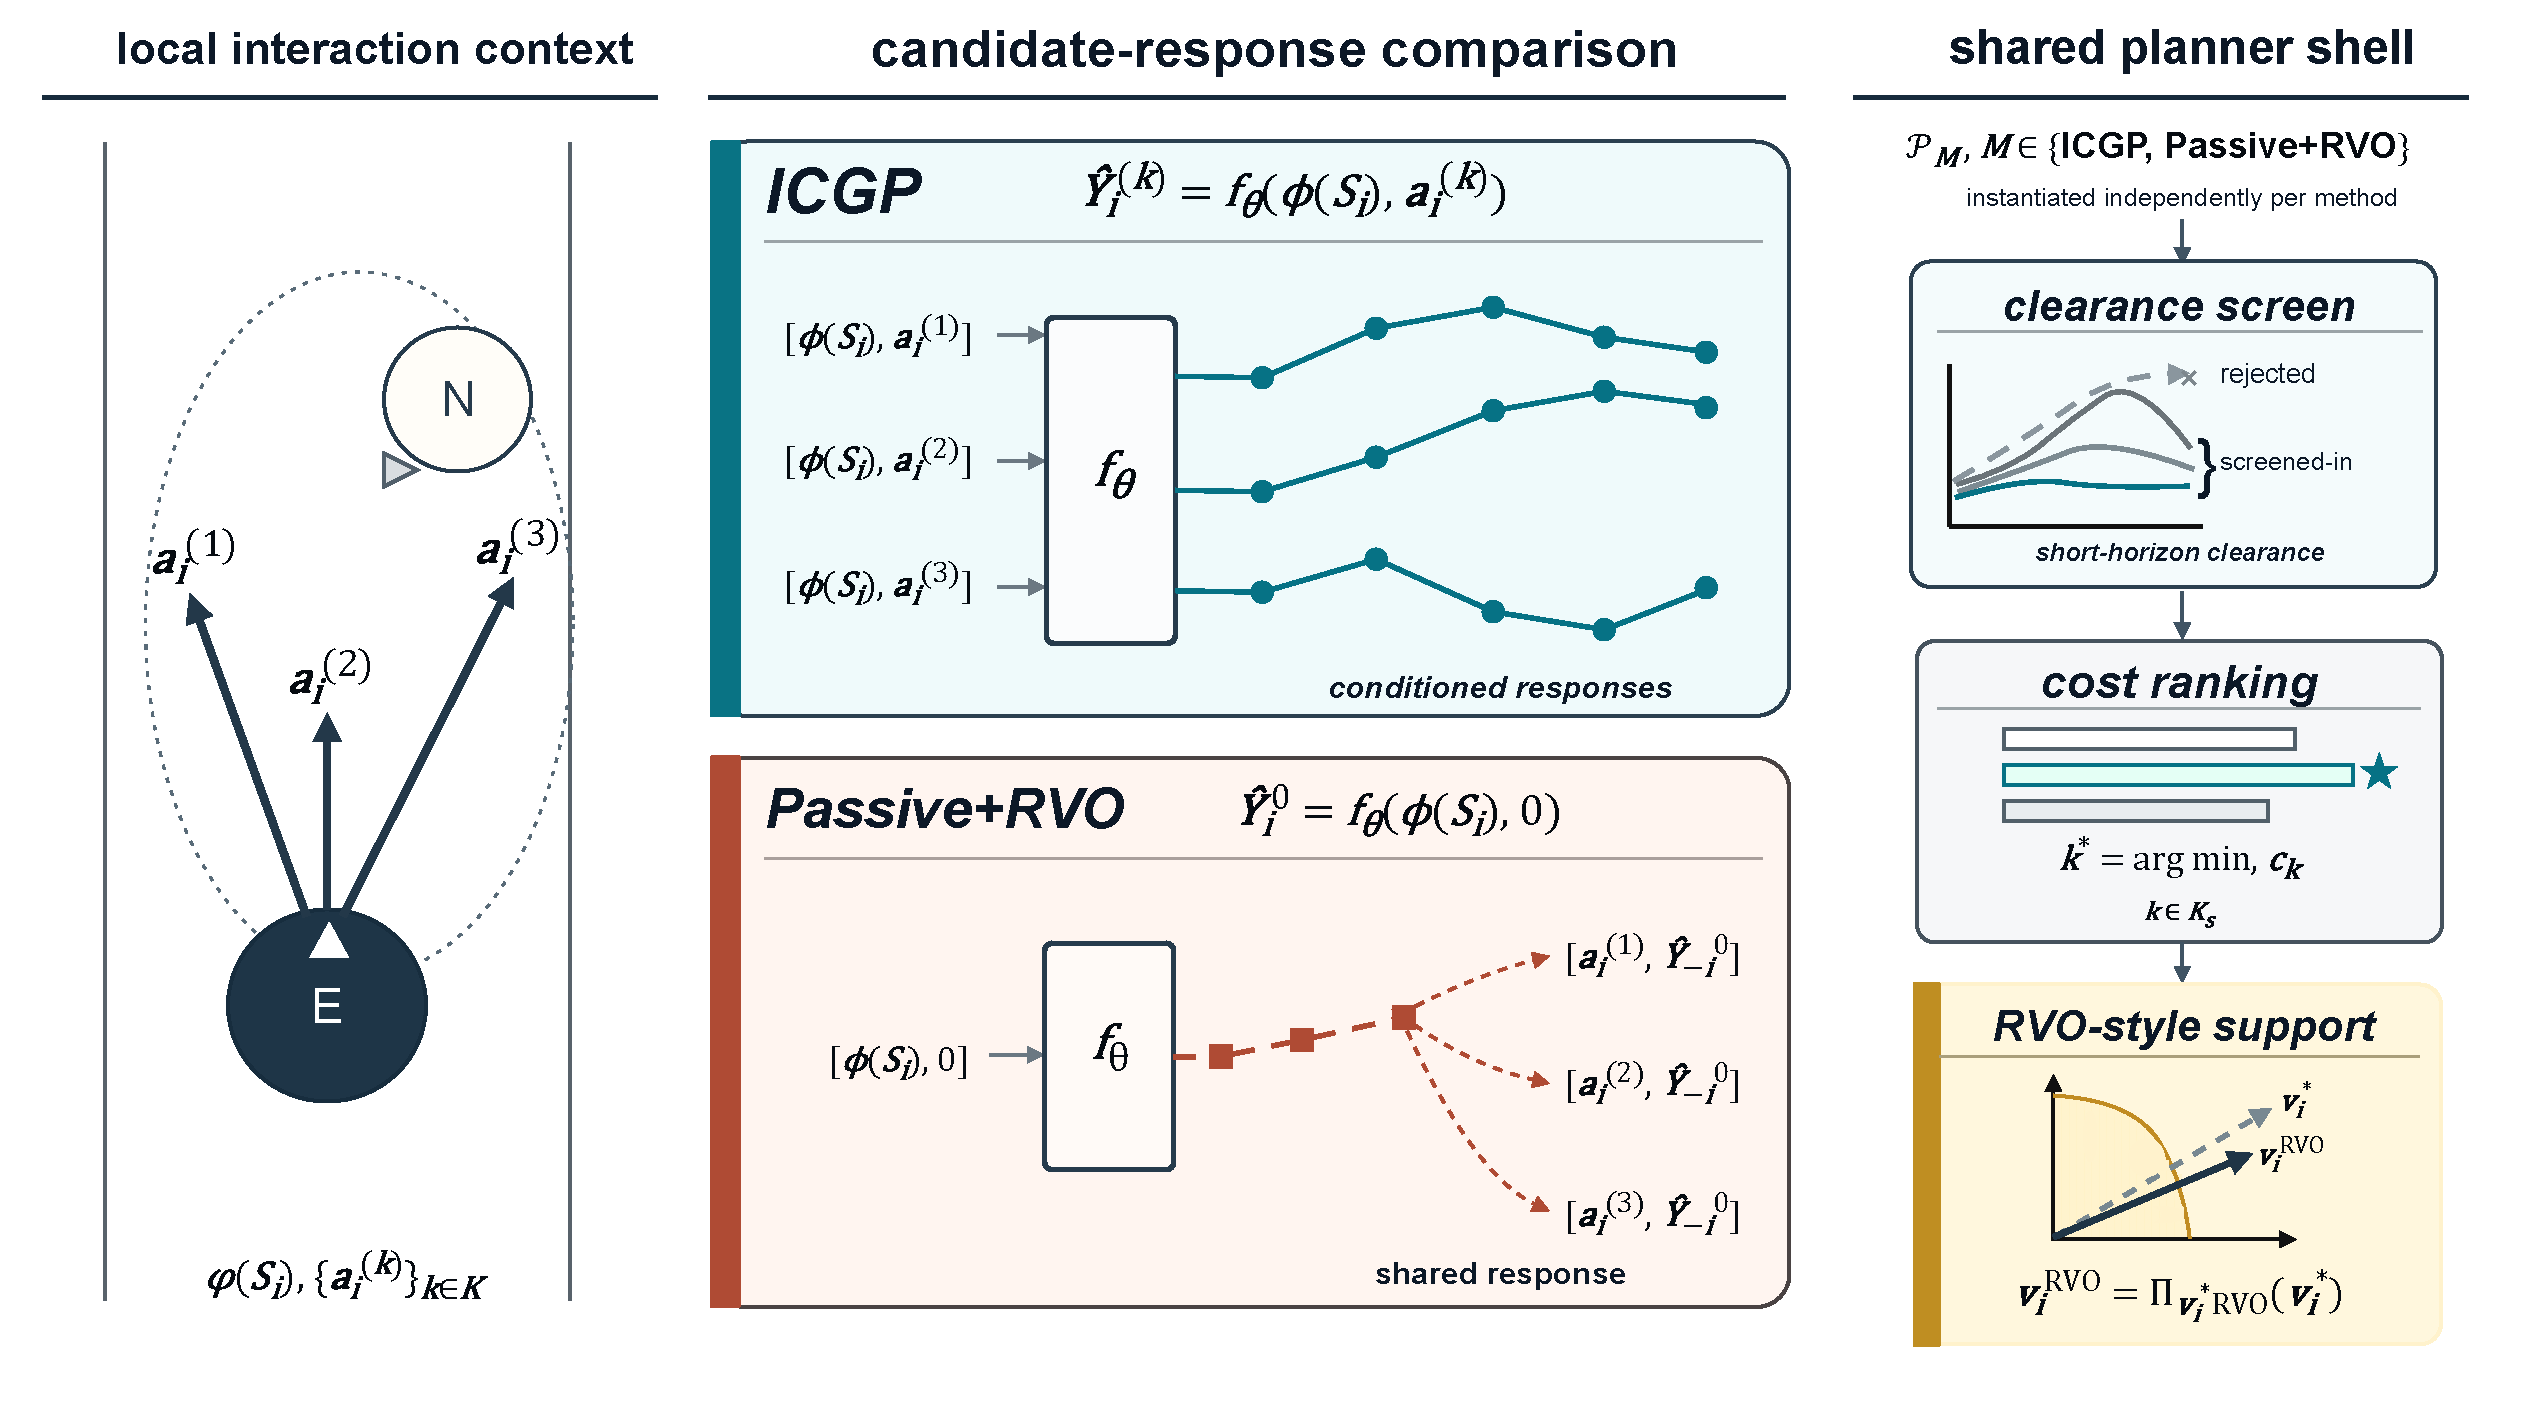
\includegraphics[width=0.90\textwidth]{Fig1.pdf}
\caption{ICGP mechanism schematic. Passive forecasting reuses one neighbor response, whereas ICGP evaluates candidate-conditioned neighbor responses, screens clearance, ranks cost, and applies an RVO-style support layer before replanning}
\label{fig:concept}
\end{figure}

\section{Experimental protocol and statistical design}
\label{sec:protocol}

\subsection{Non-pooled protocols and boundary evidence}

The legacy and formal sensitivity protocols use different sampling frames. The legacy four-map subset contains 960 method records and 240 matched ICGP--Passive cases. The separately generated sensitivity corpus replaces one map, crosses four methods with four Gaussian levels, and contains 3,840 records. Within each scenario--team-size--seed case, all methods share the pre-generated schedule. Estimates from the two corpora are not pooled.

The architecture-by-conditioning experiment retains the sensitivity maps, team sizes, Gaussian levels, seeds, and 220-step endpoint, but separately trained models and batching produce an independent 3,840-record paired corpus. The ROS~2/Gazebo diagnostic differs more substantially: it uses ten seeds, eight robots, three methods, a denser merge, and a different endpoint. We treat it as operating-boundary evidence, not as an extension of either statistical sample.

Table~\ref{tab:protocol} lists these protocols and their intended interpretations. The map names come from the local scenario-generation code; they do not denote a physical facility or public benchmark dataset.

\begin{table*}[htbp]
\caption{Protocols used in the study and the separate Gazebo boundary diagnostic. Rows are not pooled}
\label{tab:protocol}
\centering
\scriptsize
\begin{tabular}{@{}>{\raggedright\arraybackslash}p{0.16\textwidth}@{\hspace{1.1em}}>{\raggedright\arraybackslash}p{0.38\textwidth}@{\hspace{1.1em}}>{\raggedright\arraybackslash}p{0.38\textwidth}@{}}
\toprule
\textbf{Protocol} & \textbf{Design} & \textbf{Interpretation} \\
\midrule
Legacy main & Four constrained maps; 4/8 agents; 30 seeds; 960 method records & Clean-shell method comparison; separate from the noise study \\
Formal noise & Four maps; 4/8 agents; 30 paired seeds; four levels; four methods; 3,840 records & Simulation sensitivity to perturbations in neighbor observations \\
Factorial ablation & Plain/residual architecture crossed with candidate/zero query; four Gaussian levels; 3,840 records & Separates representation and query effects within a synchronized experiment \\
Auxiliary controls & Residual-passive and light-GNN protocols with 40 and 20 matched pairs & Attribution and architecture diagnostics \\
Gazebo boundary & Eight-robot merge bottleneck; ten seeds; ICGP, Passive, and Residual-passive & High-density stress diagnostic; not a superiority, sensor, or hardware claim \\
ROS 2/RViz visual trace & Four-robot merge bottleneck; one retained seed; synchronized state and planner logs & System-integration and deadlock diagnostic; separate from the ten-seed boundary \\
\bottomrule
\end{tabular}
\end{table*}

\subsection{Scenario generation and episode state}

Each scenario generator returns a bounded planar workspace, robot positions, goals, obstacle geometry, and a fixed robot count. Formal metadata records the scenario-generation and RVO-layer configurations. Every raw result also stores workspace area, agent density, area per agent, passage width, and agents per passage width. These fields are descriptive covariates; they are not post-hoc selection criteria.

The controller updates robots sequentially at every simulation step. For each ego robot, it selects nearest neighbors up to the four-slot limit. The local observation keeps the ego state exact; the current row of the pre-generated schedule replaces neighbor positions and velocities. Goals and obstacle geometry remain exact. Once all commands are selected, the simulator integrates positions and velocities, updates path length and control effort, and records collision and safety-margin events.

An episode is successful only if it reaches the goal within the configured tolerance and has no collision. Progress ratio uses mean final goal distance relative to mean initial goal distance. Completion time is the simulated time to the first state satisfying the goal condition, or the maximum duration for an incomplete episode. Minimum distance is the smallest reported clearance. A safety violation is a configured margin event, not a collision-equivalent label.

\subsection{Observation-noise schedule}

For scenario $s$, agent count $n$, episode seed $r$, and noise level $\ell$, the schedule seed is a stable hash of the protocol version, scenario name, agent count, episode seed, and level name. At each simulation step it provides an independent zero-mean Gaussian position and velocity perturbation for every robot slot. For ego robot $i$,

\begin{equation}
\widetilde{p}_j(t)=p_j(t)+\varepsilon^p_j(t),\qquad
\widetilde{v}_j(t)=v_j(t)+\varepsilon^v_j(t),\qquad j\neq i,
\label{eq:noise}
\end{equation}

with $\varepsilon^p_j(t)\sim\mathcal{N}(0,\sigma_p^2 I)$ and $\varepsilon^v_j(t)\sim\mathcal{N}(0,\sigma_v^2 I)$. The ego row is then overwritten with its true state, while the simulation state itself remains unchanged. The common-random-number construction prevents a paired ICGP--Passive difference from being driven by different noise draws.

The four levels are clean $(0.00\,\mathrm{m},0.00\,\mathrm{m/s})$, low $(0.02\,\mathrm{m},0.04\,\mathrm{m/s})$, medium $(0.05\,\mathrm{m},0.10\,\mathrm{m/s})$, and high $(0.10\,\mathrm{m},0.20\,\mathrm{m/s})$. Labels such as mild localization error, common simulation/localization error, and clearly degraded condition describe the design only; they are not calibrated specifications for a camera or localization product.

Three stress-test extensions remain separate from the Gaussian corpus. Their low and high settings use $(0.02\,\mathrm{m},0.04\,\mathrm{m/s})$ and $(0.10\,\mathrm{m},0.20\,\mathrm{m/s})$. One extension uses $\varepsilon_t=\rho\varepsilon_{t-1}+\sqrt{1-\rho^2}\,\eta_t$ with $\rho=0.85$; the other two insert short periods of zeroed neighbor rows with probability 0.05 or 0.10 and maximum duration three. Common random numbers are retained across methods. Each extension has 1,920 records, for 5,760 in total, and remains a sensitivity test rather than sensor validation.

\subsection{Prediction-quality diagnostic}

The on-policy prediction trace compares the selected-action prediction with the subsequently realized simulator trajectory. Average displacement error (ADE) averages Euclidean error over available future steps and tracked neighbors; final displacement error (FDE) uses the last available horizon step. Candidate-response spread is the coordinate standard deviation across the five candidate-conditioned predictions. The diagnostic contains 1,440 case-method-noise rows; case summaries and integrity checks are included in the supplementary data package. These are mechanism diagnostics, not additional primary estimands.

\subsection{Primary metrics and estimands}

The primary contrast is ICGP+RVO minus Passive+RVO within a matched case. Positive differences favor ICGP for progress ratio and success; negative differences favor it for completion time, final goal distance, collision, and safety violation. A positive minimum-distance difference is favorable, although minimum distance alone says nothing about goal progress.

At each noise level, the estimand is the mean paired difference over 240 matched cases. A paired analysis is appropriate because the map, robot count, episode seed, scenario realization, and noise schedule are shared. It removes part of the variation due to scenario difficulty and makes the interval a within-case comparison.

For each method and noise level, we report the mean and a percentile bootstrap 95\% confidence interval over 240 method records. For each paired metric, the confidence interval is computed from 10,000 resamples of the 240 paired differences, following the nonparametric resampling logic described by Efron and Tibshirani \cite{efron1993}. The two-sided paired sign-flip test tests whether the mean signed difference is zero. The implementation enumerates all sign assignments for at most 16 pairs and uses a seeded Monte Carlo sign-flip approximation with plus-one correction for larger samples, consistent with the permutation-testing framework of Good \cite{good2005}. The reported $p$ values are nominal, within-archive diagnostics without multiplicity correction across noise levels, metrics, and baselines; they are not familywise claims of general robustness. The formal study therefore does not use a normality assumption for the paired difference.

We report effect sizes, confidence intervals, and test values together. A small $p$ value is not presented as proof of practical importance, and a confidence interval crossing zero is not presented as proof of equivalence. The high-noise safety increase is retained even though the progress effect is also positive. The study has four noise levels and several metrics; the results are interpreted as a prespecified sensitivity profile rather than as a claim of universal robustness.

\subsection{Separate Gazebo/ROS 2 boundary diagnostic}

The retained Gazebo package contains a ten-seed, eight-robot merge-bottleneck diagnostic for ICGP, Passive, and Residual-passive. It uses a different ROS~2/Gazebo simulator, density regime, and deadlock endpoint, so it is not pooled with the 2-D protocols. The package preserves the per-run state, planner, distance, and audit records behind the reported boundary metrics. Its index covers 600 raw artifacts; an independent recomputation found no mismatch in the summary, aggregate, paired-difference, or file-hash checks.

A separate visual-support record was retained from the ROS 2/Gazebo diagnostic. It contains a real RViz GUI capture, an auxiliary Gazebo GUI capture, synchronized four-robot state and planner logs, recorded run information, and derived trajectory and time-series panels. This package is deliberately treated as a single-seed system diagnostic. It documents the integration path and a concrete multi-robot execution trace, but it is not pooled with the ten-seed boundary summary and does not support a multi-seed deadlock-rate claim.

This diagnostic is useful because it prevents an overly broad interpretation of the lower-density results. It is not a real-robot experiment, a calibrated observation study, or a matched extension of the formal noise corpus. We consequently report its unfavorable outcomes as boundary evidence and do not pool it with any paired inference in this paper.

\section{Results}
\label{sec:results}

\subsection{Legacy main comparison}

The clean legacy protocol supplies the baseline before the observation-noise experiment. In the selected four-map subset, ICGP+RVO has mean progress 0.830 and Passive+RVO 0.794. Their paired progress difference is $+0.0356$ (bootstrap 95\% CI $[0.0245,0.0467]$); the paired randomization test uses 100,000 sign flips and gives $p<0.001$ with the plus-one correction. ICGP+RVO also reduces final goal distance by $0.3738\,\mathrm{m}$ (CI $[-0.4895,-0.2583]$) under the same paired convention.

Reactive RVO reaches mean progress 0.836 and final goal distance 1.716 m, so ICGP+RVO is not the highest-progress method in this protocol. The ICGP--Passive contrast concerns candidate-conditioned prediction within the learned-planning shell; it does not establish dominance over reactive control. Collision rates are 0.013 for both methods at the displayed precision. ICGP's safety-violation mean is 0.104 versus 0.129 for Passive+RVO, but the paired interval includes zero. The legacy comparison therefore indicates efficiency and goal-distance differences, not uniform safety improvement.

Figure~\ref{fig:main} shows the two primary means with method-level bootstrap intervals. The auxiliary controls use separate records and are not pooled with the formal noise experiment. In the clean auxiliary protocol, ICGP exceeds residual-passive by 0.0689 over 40 matched pairs and a lightweight graph control by 0.0488 over 20 matched pairs. These smaller protocols have their own logged configurations.

\begin{figure}[htbp]
\centering
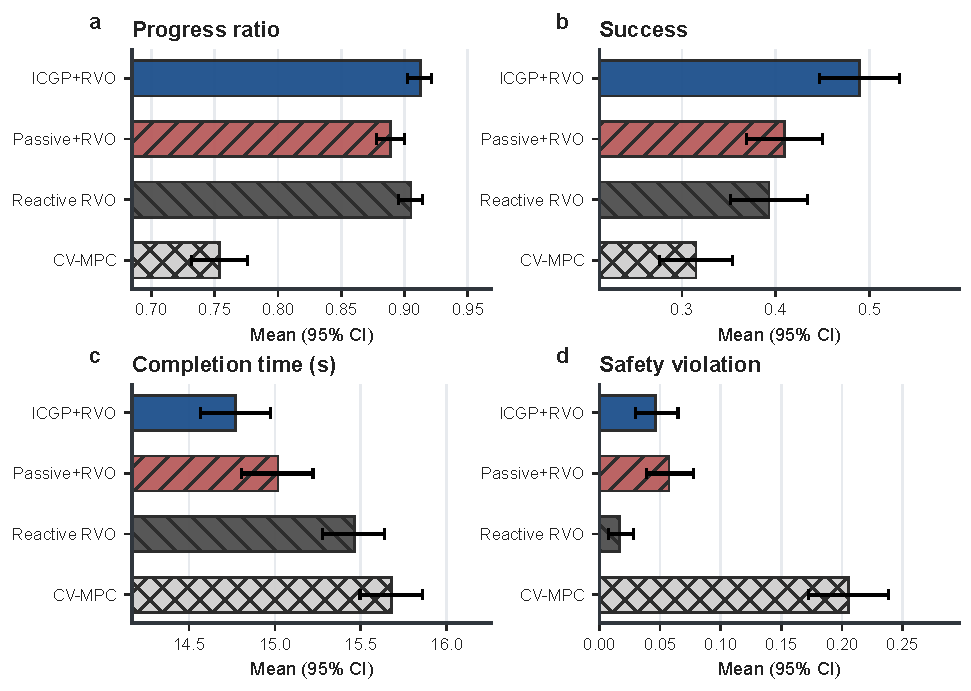
\includegraphics[width=\textwidth]{Fig2.pdf}
\caption{Legacy main outcomes. Horizontal bars show method means with bootstrap intervals; paired ICGP--Passive statistics are reported in the text}
\label{fig:main}
\end{figure}

\subsection{Gazebo boundary result}

Across ten Gazebo/ROS~2 seeds, mean progress was 0.371 for ICGP and 0.403 for Passive, a paired difference of $-0.0318$. Terminal deadlock occurred in all ten ICGP runs, nine Passive runs, and all ten Residual-passive runs. All 30 runs were collision-free, although one ICGP run crossed the configured safety-distance threshold and reached a minimum distance of $0.496\,\mathrm{m}$. This is a finite-horizon deadlock case in a symmetric merge.
The supplementary data package groups the boundary summary, synchronized logs, GUI captures, derived panels, and validation summary. Log-derived traces come from synchronized logs; screenshots provide visual support only.

\subsection{Formal observation-noise sensitivity}

Reactive RVO provides an almost flat progress reference in the Gaussian experiment, with means from 0.936 to 0.939 (Fig.~\ref{fig:noise}). The learned comparison is less regular. ICGP's largest progress difference from Passive occurs at low noise ($+0.0153$); at the medium level it is $+0.0021$. Only the low- and high-noise intervals exclude zero ($p=0.0052$ and $0.0041$). The four points do not define a dose--response relation, and these records do not identify the cause of the non-monotone pattern.

Completion time favors ICGP at all four levels, with paired reductions from $0.62$ to $0.89\,\mathrm{s}$. Success is less stable: the low-noise increase is 7.92 percentage points, while the medium estimate is unresolved. These are episode-level simulation measures, not fleet-throughput measures.

At the upper endpoint, ICGP finishes $0.72\,\mathrm{s}$ sooner while its configured-margin event rate is 5.00 percentage points higher (95\% CI $[+0.83,+9.17]$; $p=0.0247$). The safety intervals at the other settings include zero. The faster completion and adverse margin estimate occur in the same condition, but the paired data do not establish a causal link between them.

Table~\ref{tab:noise} reports the paired estimates, confidence intervals, and sign-flip tests. Figure~\ref{fig:heterogeneity} then resolves the high-noise completion-time and safety differences by scenario and team size.
\begin{figure}[htbp]
\centering
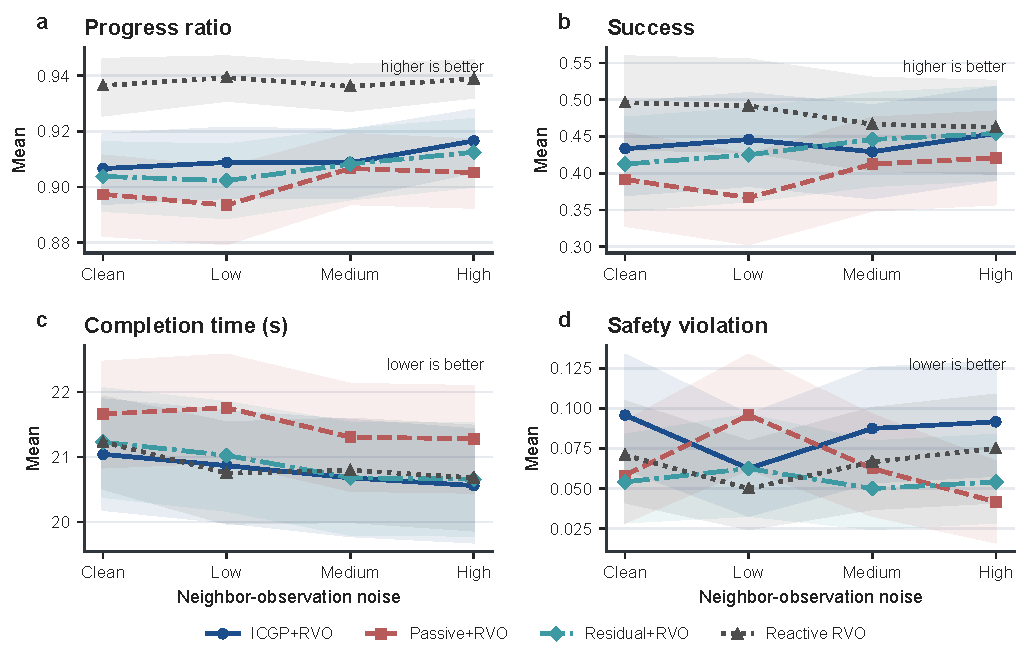
\includegraphics[width=\textwidth]{Fig3.pdf}
\caption{Formal neighbor-observation sensitivity. Points show method means over 240 episodes per method and level; intervals are percentile-bootstrap 95\%}
\label{fig:noise}
\end{figure}

\begin{figure}[htbp]
\centering
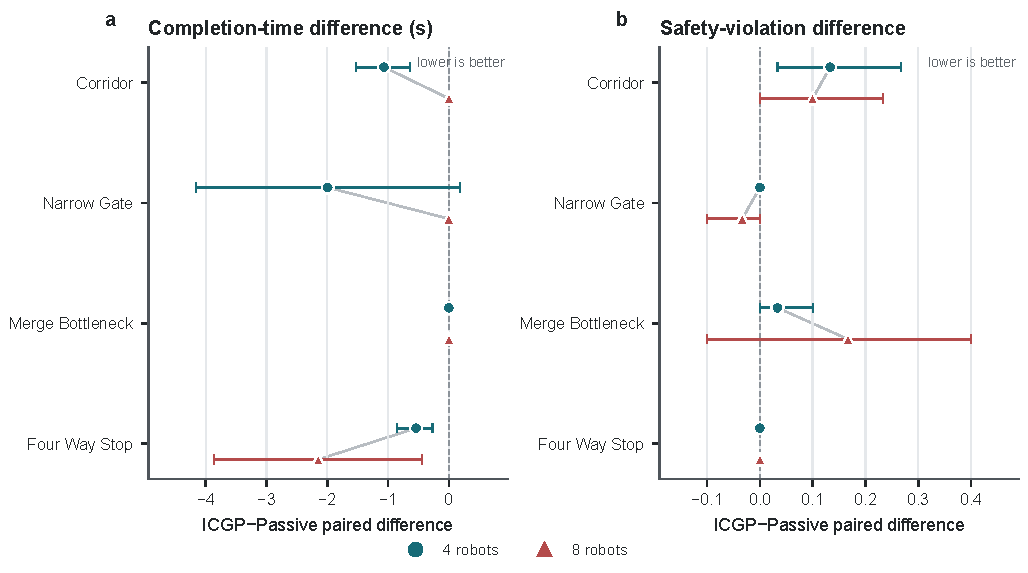
\includegraphics[width=\textwidth]{Fig4.pdf}
\caption{Scenario and team-size paired interaction. Circles and triangles denote 4- and 8-robot cases, respectively. Each marker shows the ICGP+RVO minus Passive+RVO difference for 30 matched seeds in a scenario--team-size cell; error bars are percentile-bootstrap 95\% intervals. The panel is descriptive only}
\label{fig:heterogeneity}
\end{figure}

\begin{table*}[htbp]
\caption{Primary paired observation-noise results over 240 matched cases per condition. Rows separate the ICGP+RVO minus Passive+RVO mean difference, 95\% percentile-bootstrap interval, and two-sided paired sign-flip $p$ value. Success and safety differences are in percentage points; positive safety differences are adverse}
\label{tab:noise}
\centering
\scriptsize
\setlength{\tabcolsep}{3pt}
\renewcommand{\arraystretch}{0.96}
\begin{tabular}{@{}p{0.125\textwidth}p{0.098\textwidth}p{0.1525\textwidth}p{0.1525\textwidth}p{0.1525\textwidth}p{0.1525\textwidth}@{}}
\toprule
Outcome & Statistic & Clean $(0,0)$ & Low $(0.02,0.04)$ & Medium $(0.05,0.10)$ & High $(0.10,0.20)$ \\
\midrule
Progress & Estimate & $+0.0092$ & $+0.0153$ & $+0.0021$ & $+0.0114$ \\
 & 95\% CI & $[-0.0019,\allowbreak 0.0203]$ & $[0.0045,\allowbreak 0.0261]$ & $[-0.0059,\allowbreak 0.0103]$ & $[0.0039,\allowbreak 0.0193]$ \\
 & $p$ & 0.1063 & 0.0052 & 0.6196 & 0.0041 \\
\addlinespace[2pt]
Success & Estimate & $+4.17$ & $+7.92$ & $+1.67$ & $+3.33$ \\
 & 95\% CI & $[0.42,\allowbreak 7.92]$ & $[3.75,\allowbreak 12.08]$ & $[-1.67,\allowbreak 5.00]$ & $[0.00,\allowbreak 6.67]$ \\
 & $p$ & 0.0435 & 0.0001 & 0.4866 & 0.0983 \\
\addlinespace[2pt]
Safety violation & Estimate & $+3.75$ & $-3.33$ & $+2.50$ & $+5.00$ \\
 & 95\% CI & $[-0.42,\allowbreak 7.92]$ & $[-7.50,\allowbreak 0.83]$ & $[-2.50,\allowbreak 7.50]$ & $[0.83,\allowbreak 9.17]$ \\
 & $p$ & 0.1369 & 0.1627 & 0.4114 & 0.0247 \\
\addlinespace[2pt]
Completion time (s) & Estimate & $-0.62$ & $-0.89$ & $-0.63$ & $-0.72$ \\
 & 95\% CI & $[-1.05,\allowbreak -0.20]$ & $[-1.31,\allowbreak -0.49]$ & $[-1.00,\allowbreak -0.26]$ & $[-1.10,\allowbreak -0.35]$ \\
 & $p$ & 0.0053 & 0.0001 & 0.0007 & 0.0001 \\
\bottomrule
\end{tabular}
\end{table*}

Method-level means are consistent with the paired results. ICGP has higher progress than Passive at all four levels, with only a small difference at medium noise. Residual-passive is close to ICGP in progress and has lower safety-violation means in the clean and medium conditions. Reactive RVO has the highest progress and lower safety-violation means in the clean, low, and medium conditions. No method is best on every outcome.
\subsection{Secondary outcomes and engineering quantities}

The paired records also contain final goal distance. ICGP is closer to the goal by $0.1604\,\mathrm{m}$ at low noise (95\% CI $[-0.2757,-0.0485]$, $p=0.0062$) and by $0.1189\,\mathrm{m}$ at high noise (95\% CI $[-0.2012,-0.0392]$, $p=0.0056$). The clean difference is smaller, $-0.0967\,\mathrm{m}$, with an interval crossing zero ($p=0.1106$); the medium difference is $-0.0227\,\mathrm{m}$ ($p=0.6093$). These values track the non-monotone progress profile rather than a single binary success threshold.

Collision and minimum-distance metrics do not show a corresponding safety improvement. Collision differences are zero in the clean condition, +0.83 percentage points at low noise, +1.25 points at medium noise, and +2.08 points at high noise; all four paired intervals include zero. Minimum-distance differences are +0.0043, +0.0115, $-0.0003$, and $-0.0051\,\mathrm{m}$ from clean through high noise, with none excluding zero. The configured safety-violation flag is therefore the more sensitive adverse signal at high noise, but it is not equivalent to collision or to a formal distance guarantee.

\subsection{Fully crossed architecture-by-conditioning ablation}
\label{sec:factorial-ablation}

The factorial corpus contains 3,840 records with no missing case--method key. Generated training examples, optimizer, width, dropout, candidate set, screen, cost, RVO layer, Gaussian schedules, and the 240 paired cases per noise level are fixed. Only the parameterization (plain or residual) and the action input (nonzero or zero) vary. This synchronized design tests the attribution implied by the historical residual-candidate versus plain-zero comparison.

Candidate-minus-zero progress intervals cross zero for both architectures at every Gaussian level. Completion time is more sensitive, but its pattern depends on architecture. The plain-model estimate favors candidate input most strongly at medium noise ($-0.877\,\mathrm{s}$), whereas the residual estimate is $-0.023\,\mathrm{s}$. Their difference is $+0.855\,\mathrm{s}$ (95\% CI $[+0.260,+1.466]\,\mathrm{s}$, $p=0.0069$). Residual zero also has a negative time estimate relative to plain zero at every level, although its clean-condition interval crosses zero. The historical contrast cannot therefore be assigned to a common, architecture-independent conditioning effect.

Table~\ref{tab:factorial-time} summarizes these completion-time contrasts across the four Gaussian conditions.

\begin{table*}[htbp]
\caption{Completion-time effects from the fully crossed ablation over 240 matched cases per Gaussian condition. Columns give $(\sigma_p,\sigma_v)$ in m and m/s. Values are paired mean differences in seconds; negative values favor the first named condition. The interaction subtracts the plain candidate effect from the residual candidate effect}
\label{tab:factorial-time}
\centering
\small
\begin{tabular}{@{}lrrrr@{}}
\toprule
Comparison & $(0,0)$ & $(0.02,0.04)$ & $(0.05,0.10)$ & $(0.10,0.20)$ \\
\midrule
Candidate minus zero, plain model & $-0.454$ & $-0.505$ & $-0.877$ & $-0.431$ \\
Candidate minus zero, residual model & $-0.375$ & $-0.012$ & $-0.023$ & $-0.417$ \\
Residual minus plain, zero query & $-0.465$ & $-0.593$ & $-0.987$ & $-0.493$ \\
Architecture-by-query interaction & $+0.079$ & $+0.493$ & $+0.855$ & $+0.014$ \\
\bottomrule
\end{tabular}
\end{table*}

Residual candidate raises the clean-condition safety-violation rate by 3.75 percentage points relative to residual zero (95\% CI $[+0.83,+7.08]$); every other interval in that comparison crosses zero. Held-out ADE and FDE likewise do not favor candidate input within either architecture. These controls do not support the stronger claim that conditioning is the principal source of the original ICGP--Passive difference.

Table~\ref{tab:factorial-diagnostics} gives the execution context. Residual cells reject fewer candidates and trigger fewer RVO interventions on average than plain cells, at about $1.28\times$ the plain-zero model-side time. Adding candidate input changes neither timing nor intervention frequency substantially. These episode means do not explain the progress ordering because the records omit pre/post-projection vectors, curvature, and terminal-deadlock labels.

\begin{table}[htbp]
\caption{Factorial-ablation engineering diagnostics over 960 records per cell. Parentheses contain all-rejected rates; timing covers only the model forward pass and is reported as the mean $\pm$ sample standard deviation of per-episode decision means}
\label{tab:factorial-diagnostics}
\centering
\scriptsize
\begin{tabular}{@{}l r c r r@{}}
\toprule
Cell & Reject (all) (\%) & RVO intervention (\%) & $t_{\mathrm{model}}$ (ms) & Relative \\
\midrule
Plain candidate & 39.07 (21.36) & 65.52 & $0.149\pm0.056$ & $1.00\times$ \\
Plain zero & 38.37 (23.45) & 65.46 & $0.149\pm0.058$ & $1.00\times$ \\
Residual candidate & 36.36 (19.40) & 62.58 & $0.190\pm0.073$ & $1.28\times$ \\
Residual zero & 35.62 (20.09) & 63.62 & $0.191\pm0.074$ & $1.28\times$ \\
\bottomrule
\end{tabular}
\end{table}

\subsection{Extended simulation stress tests}
\label{sec:stress-tests}

The stress tests replace independent Gaussian perturbations with a temporally correlated AR(1) schedule or short periods of zeroed neighbor observations. Each row is an ICGP+RVO minus Passive+RVO difference over 240 matched cases. We report these protocols separately because they change the observation process. Figure~\ref{fig:stress} shows the paired distributions and Table~\ref{tab:stress} gives the completion-time estimates and tests.

\begin{figure}[htbp]
\centering
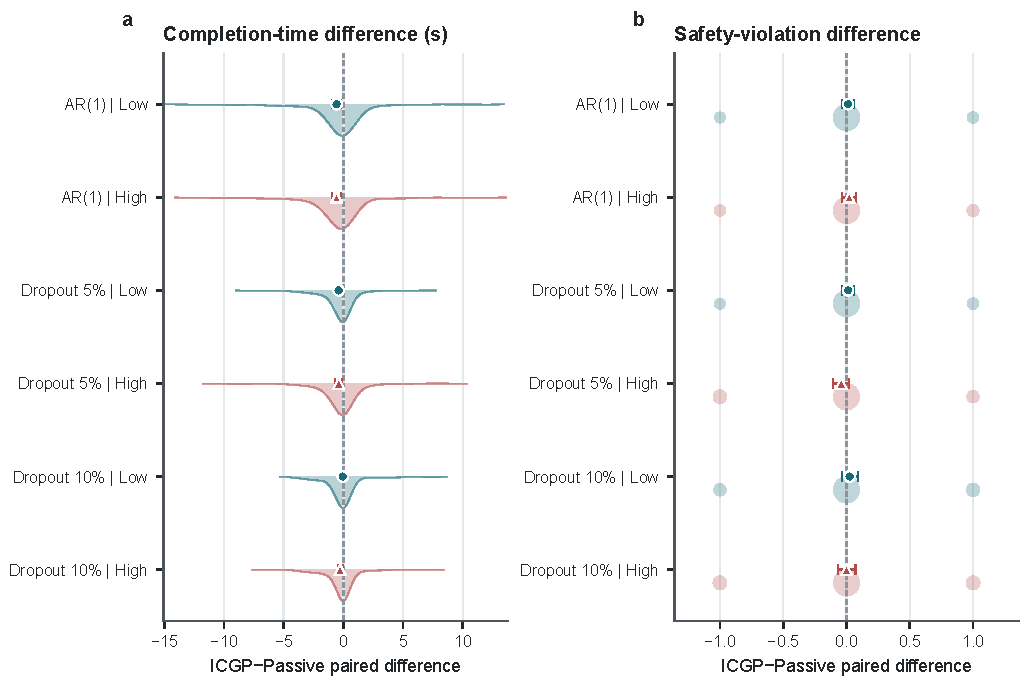
\includegraphics[width=\textwidth]{Fig5.pdf}
\caption{Paired distribution atlas for completion time and safety violation under temporally correlated and dropout observations. Panels report the raw ICGP+RVO minus Passive+RVO deltas together with means and percentile-bootstrap 95\% intervals. Rows separate AR(1) noise and dropout protocols at low and high levels}
\label{fig:stress}
\end{figure}

\begin{table*}[htbp]
\caption{Extended stress-test summary over 240 matched cases per condition. Completion-time cells report ICGP+RVO minus Passive+RVO differences with percentile-bootstrap 95\% intervals and nominal paired sign-flip $p$ values. The full metric grid is retained in the supplementary data}
\label{tab:stress}
\centering
\scriptsize
\setlength{\tabcolsep}{5pt}
\begin{tabular}{@{}>{\raggedright\arraybackslash}p{0.17\textwidth}>{\raggedright\arraybackslash}p{0.25\textwidth}>{\raggedright\arraybackslash}p{0.25\textwidth}>{\raggedright\arraybackslash}p{0.24\textwidth}@{}}
\toprule
Protocol & Low completion-time difference (s) & High completion-time difference (s) & Other paired outcomes \\
\midrule
AR(1), $\rho=0.85$ & $-0.571$; CI $[-0.971,-0.190]$; $p=0.0045$ & $-0.580$; CI $[-0.979,-0.185]$; $p=0.0037$ & Progress and safety intervals include zero \\
Dropout, $p=0.05$ & $-0.396$; CI $[-0.629,-0.176]$; $p=0.0005$ & $-0.388$; CI $[-0.686,-0.094]$; $p=0.0109$ & Progress and safety intervals include zero \\
Dropout, $p=0.10$ & $-0.049$; CI $[-0.274,+0.188]$; $p=0.6836$ & $-0.271$; CI $[-0.473,-0.064]$; $p=0.0080$ & Progress and safety intervals include zero \\
\bottomrule
\end{tabular}
\end{table*}

Completion-time intervals exclude zero at both AR(1) levels, both $p=0.05$ dropout levels, and the high $p=0.10$ level; the low $p=0.10$ condition is inconclusive. Progress and safety-violation intervals include zero in all six conditions, and collision and minimum-distance summaries show no consistent separation. The extensions therefore support a completion-time effect only, not a general progress or safety effect.

\subsection{Prediction-quality analysis}
\label{sec:prediction-quality}

The on-policy diagnostic evaluates the response model after candidate selection. It covers 240 matched cases in each clean and high-noise condition and averages error over the available future horizon. Figure~\ref{fig:prediction-quality} and Table~\ref{tab:prediction-quality} show lower ADE and FDE for ICGP than for Passive. Paired ADE differences are $-0.2750$ (95\% CI $[-0.3072,-0.2440]$) in the clean condition and $-0.2837$ (95\% CI $[-0.3124,-0.2553]$) under high noise. The corresponding FDE differences are $-0.3026$ (95\% CI $[-0.3364,-0.2702]$) and $-0.3167$ (95\% CI $[-0.3459,-0.2872]$). These values describe selected-action prediction inside the simulator.

ICGP produces a candidate-response spread of 0.1288 in the clean condition and 0.1284 under high noise; Passive and Residual-passive have zero spread in this diagnostic. The response thus changes with the candidate, and selected-action error is lower. The residual comparison remains close under high noise, so these diagnostics do not resolve either the link to planning outcomes or the attribution among candidate information, parameterization, and training.
\begin{figure}[htbp]
\centering
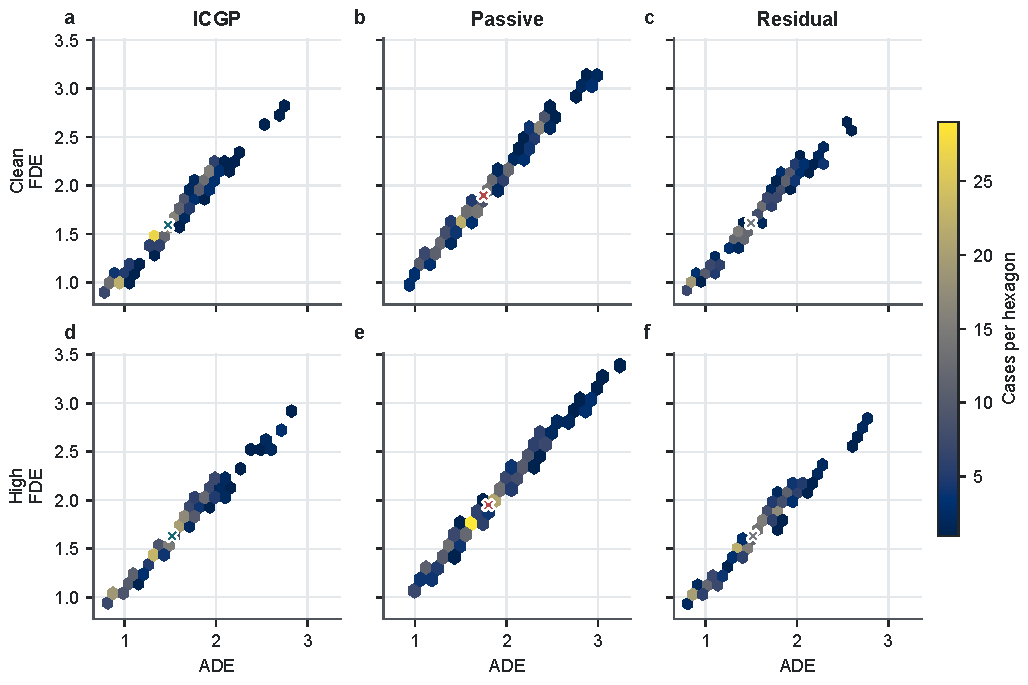
\includegraphics[width=\textwidth]{Fig6.pdf}
\caption{Joint average displacement error (ADE) and final displacement error (FDE) hexbin densities. Panels (a)--(c) show clean-condition ICGP, Passive, and Residual-passive results; panels (d)--(f) show the corresponding high-noise results. Crosses mark method means, and the shared luminance scale reports cases per hexagon}
\label{fig:prediction-quality}
\end{figure}

The quantitative results are accompanied by a ROS~2/Gazebo/RViz system view. Figure~\ref{fig:simulation-rollouts} combines an RViz capture with a four-robot merge trajectory and time-resolved diagnostics reconstructed from synchronized logs. This single-seed integration record documents the execution path; it is not an additional statistical sample and does not alter the formal estimates.
\begin{figure}[htbp]
\centering
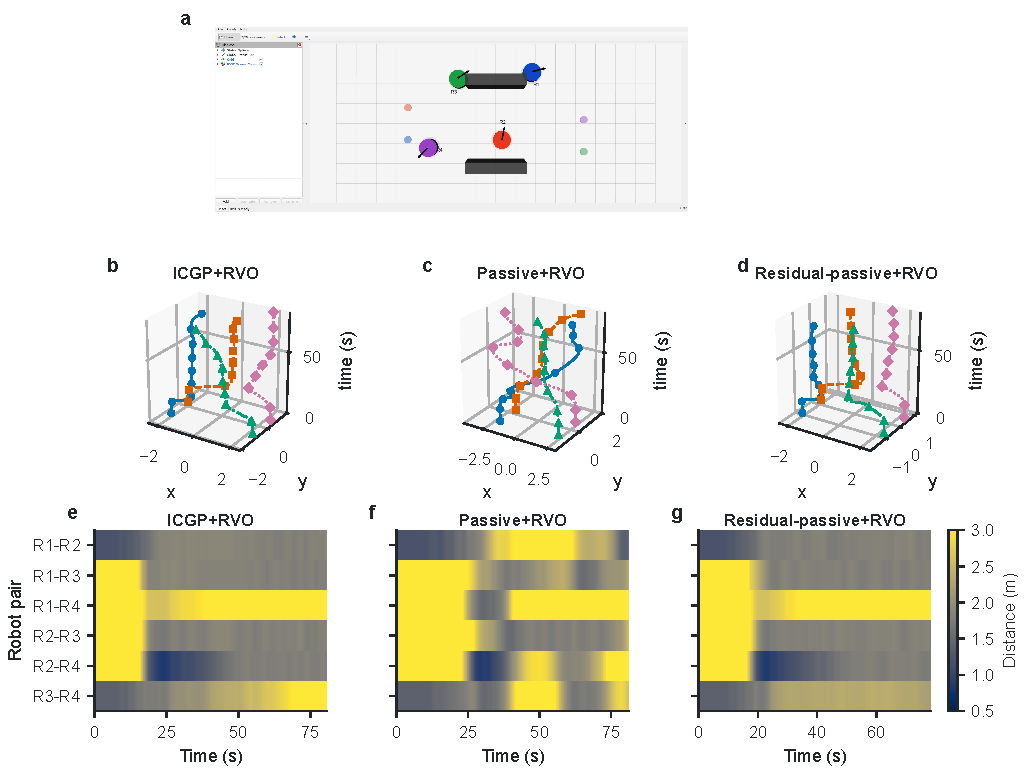
\includegraphics[width=\textwidth]{Fig7.pdf}
\caption{ROS~2/Gazebo/RViz merge-bottleneck diagnostic. Panel (a) is a retained RViz screenshot; panels (b)--(d) show log-derived three-dimensional space--time paths for ICGP+RVO, Passive+RVO, and Residual-passive+RVO; panels (e)--(g) show pairwise-clearance heatmaps with a distance scale. Robot identity is redundantly encoded by line style and periodic marker. This single-seed diagnostic is not pooled with the formal estimates}
\label{fig:simulation-rollouts}
\end{figure}

\begin{table*}[htbp]
\caption{On-policy prediction-quality means. Each row contains 240 case summaries. ADE and FDE are in simulator distance units; candidate spread is the mean coordinate standard deviation across the five candidate-conditioned predictions}
\label{tab:prediction-quality}
\centering
\scriptsize
\renewcommand{\arraystretch}{1.08}
\begin{tabular}{@{}llrrrr@{}}
\toprule
\multicolumn{2}{c}{Condition} & \multicolumn{4}{c}{Prediction and candidate-response diagnostics} \\
\cmidrule(lr){1-2}\cmidrule(lr){3-6}
Noise & Method & ADE & FDE & Candidate spread & Effective horizon \\
\midrule
Clean & ICGP+RVO & 1.4712 & 1.5913 & 0.1288 & 7.8174 \\
 & Passive+RVO & 1.7462 & 1.8940 & 0.0000 & 7.8254 \\
 & Residual-passive+RVO & 1.4970 & 1.6119 & 0.0000 & 7.8200 \\
High & ICGP+RVO & 1.5187 & 1.6339 & 0.1284 & 7.8113 \\
 & Passive+RVO & 1.8023 & 1.9507 & 0.0000 & 7.8210 \\
 & Residual-passive+RVO & 1.5193 & 1.6330 & 0.0000 & 7.8125 \\
\bottomrule
\end{tabular}
\end{table*}

The raw logs also record planner-side quantities that distinguish a better outcome from a changed execution pattern. Selected, predicted, and run-time margins are separate fields, as are candidate rejection, all-rejected recovery, RVO intervention, path length, control effort, smoothness, and model-side latency. We do not combine them into a post-hoc score. A controller can improve progress by selecting a more direct action, rejecting more candidates, or relying more heavily on the support layer; those mechanisms have different implications even when final progress ratios match.

In method summaries, ICGP's mean completion time is lower than Passive's at every level, while the progress ordering is usually Reactive RVO, ICGP, Residual-passive, and Passive. The ICGP--Passive gap is thus not a universal reduction in every cost. Residual-passive is close to ICGP in progress but has lower safety-violation means in the clean and medium conditions. We therefore report it separately rather than as another replicate of the primary baseline.

The timing field covers one batched forward pass. The evaluator divides the elapsed time by five candidate rows and adds that per-row value once per candidate, so the returned per-step field is effectively the batched inference time. It omits operating-system scheduling, simulator overhead, sensor acquisition, communication, and robot middleware. It can reveal changes in batching or model loading, but not hardware real-time feasibility.

Screening fields answer a different question. Reject rate counts candidate rows that fail the configured margin, not unsafe episodes, and the all-rejected flag records use of the recovery rule rather than collision. Minimum predicted and run-time margins also belong to different checker stages. Keeping these fields separate supports a later mechanism study without treating any one as a safety certificate.

\subsection{Exploratory heterogeneity by map and team size}

The aggregate paired estimate averages over four maps and two robot counts. Although this is the prespecified estimand, it can hide geometric variation. We therefore inspect paired differences within each scenario--robot-count cell, with 30 seed pairs per cell. These slices are descriptive: they did not guide map selection or controller tuning, and we make no additional uncorrected cell-wise claims.

The low-noise progress profile illustrates the spread. In the four-robot narrow-gate map, the mean ICGP--Passive difference is +0.0753, much larger than the aggregate low-noise difference of +0.0153. With eight robots in the same map, the descriptive difference is $-0.0089$. Corridor cells are near zero at both team sizes ($-0.0010$ and $-0.0020$); merge-bottleneck cells are positive (+0.0192 and +0.0359), and four-way-stop cells are also near zero (+0.0002 and +0.0039). One plausible explanation is that conditional responses help when a small action change determines whether a narrow passage remains open, but this remains a geometric hypothesis, not an identified mechanism.

The high-noise safety profile is also uneven. Corridor cells show adverse safety-violation differences of about +13.3 percentage points for four robots and +10.0 for eight. The eight-robot merge-bottleneck cell is about +16.7 points, versus +3.3 for four robots. Both four-way-stop cells are zero at the displayed precision, and the eight-robot narrow gate slightly favors ICGP (about $-3.3$ points). These cells account for the positive overall high-noise safety difference without showing that every map is less safe. They motivate a stratified follow-up with a prespecified interaction model and multiplicity control.

Robot count changes more than the number of observation rows: it alters the density of relevant neighbors, frequency of reciprocal encounters, time spent in constrained passages, and likelihood that one robot changes another's feasible set. The predictor still receives at most four neighbor rows. The eight-robot result therefore tests a denser operating point within the same local representation, not an unlimited-neighborhood planner. The archive contains density covariates for a later interaction model, but the primary comparison remains pooled over the prespecified map and team-size factors.

Noise level also interacts with geometry non-monotonically. A perturbation that is harmless in an open corridor can change the ranking of nearly equivalent actions at a merge or gate. Conversely, a constrained map may invoke the RVO layer often enough to mask a change in learned ranking. The aggregate curves should therefore not be read as a dose--response law. The four labels identify controlled perturbation magnitudes, not a universal physical-robot threshold.

We use the cell inspection to specify the next experiment, not to broaden the current claim. A follow-up should pre-register a map-by-density interaction, retain the common-random-number schedule, and report hierarchical intervals or multiplicity-adjusted tests. It should also vary the neighborhood limit and include correlated and temporally filtered errors. This would help distinguish a geometry-specific high-noise cost from one associated with the candidate-conditioned response mechanism.

Figure~\ref{fig:heterogeneity} shows this descriptive boundary without treating
the cell slices as a second inferential study. The eight-robot merge-bottleneck
cell has the largest adverse high-noise safety difference, while the completion-
time effect varies by geometry. The pooled estimate is therefore informative
for the prespecified protocol but insufficient to define a universal operating
threshold.

\subsection{Attribution, geometry, and engineering diagnostics}

Because the crossed ablation links the completion-time pattern to architecture, the following diagnostics describe the assembled implementations rather than an isolated signature of candidate conditioning.

Reactive RVO sets a second boundary. It has higher progress at every formal level, so the learned mechanism is a candidate-ranking component, not a globally superior controller. In Table~\ref{tab:planner-diagnostics}, ICGP rejects slightly fewer candidates than Passive while reaching essentially the same RVO intervention rate. Reactive RVO performs neither learned ranking nor screening and is intervened on less often. The intervention bit cannot explain these differences because the logs contain no unprojected command magnitude, angular change, or curvature.

\begin{table}[htbp]
\caption{Descriptive planner diagnostics from the 3,840-record formal Gaussian corpus. Entries are means of episode-level decision rates over 960 records per method. Candidate-screen columns do not apply to Reactive RVO}
\label{tab:planner-diagnostics}
\centering
\small
\begin{tabular}{@{}lrrr@{}}
\toprule
Method & Reject (\%) & All rejected (\%) & RVO intervention (\%) \\
\midrule
ICGP+RVO & 34.98 & 18.59 & 66.93 \\
Passive+RVO & 37.28 & 21.31 & 67.02 \\
Residual-passive+RVO & 34.83 & 19.58 & 67.53 \\
Reactive RVO & -- & -- & 56.45 \\
\bottomrule
\end{tabular}
\end{table}

The map-by-team-size panels suggest a narrow, provisional operating geometry: a gate or merge where a small action change can keep a local passage open. Even there, 30-seed cells do not establish a stable benefit, and the eight-robot setting still exposes only four neighbors. ICGP's descriptive rejection rate rises from 21.42\% with four robots to 48.54\% with eight; RVO intervention rises from 59.78\% to 74.09\%. Density and scenario evolution change together, so the four-neighbor cap cannot be isolated as the cause.

With five candidates, four neighbors, and eight predicted steps, the residual candidate-conditioned model takes $1.03\times$ the Passive model-side time (Table~\ref{tab:latency}). Reactive RVO has no learned forward pass, but the empty stored field is not an end-to-end timing advantage. Feature construction, screening, RVO, integration, sensing, transport, and operating-system jitter are outside this measurement.

\begin{table}[htbp]
\caption{Model-side inference latency in the formal Gaussian corpus. Values are the mean $\pm$ sample standard deviation of 960 episode-level means per method; relative latency uses Passive+RVO as the reference}
\label{tab:latency}
\centering
\small
\begin{tabular}{@{}lrr@{}}
\toprule
Method & $t_{\mathrm{model}}$ (ms/decision) & Relative to Passive \\
\midrule
ICGP+RVO & $14.03 \pm 7.35$ & $1.03\times$ \\
Passive+RVO & $13.62 \pm 7.32$ & $1.00\times$ \\
Residual-passive+RVO & $13.59 \pm 7.41$ & $1.00\times$ \\
Reactive RVO & -- & -- \\
\bottomrule
\end{tabular}
\end{table}

The frozen implementation batches five candidates and predicts an eight-step trajectory for four neighbors. Storage grows with candidate count, horizon, and neighbor limit, but no controlled sweep varied those quantities. A scalability claim would require fixed hardware, warm-up, numerical precision, model width, and decision workload.

\section{Discussion}
\label{sec:discussion}

\subsection{Efficiency and safety}

Within the shared learned-planning shell, completion time is the most stable difference. Its paired estimate favors ICGP across the Gaussian grid and under the moderate temporal perturbations, whereas progress is non-monotone and nearly matches Passive at the medium level. Geometry and downstream projection could contribute, but the logs contain neither candidate-rank disagreement nor projection distortion to test that explanation.

At the upper Gaussian endpoint, the $0.72\,\mathrm{s}$ completion improvement accompanies a 5.00-percentage-point rise in configured safety violations. Collision and minimum distance provide no compensating gain. A single score would hide this trade-off and would require a deployment-specific valuation of time, clearance, and failure.

\subsection{Mechanism and attribution}

The on-policy trace confirms that candidate input reaches the response output, and selected-action ADE/FDE is lower than Passive's. The synchronized ablation addresses attribution more directly. It finds no separated progress effect of candidate input within either architecture, while residual structure changes completion time and interacts with the query at medium noise. The empirical unit is consequently the assembled residual candidate-conditioned planner, not the candidate branch alone.

Reactive RVO also reaches greater progress without learned response ranking. The contribution is therefore located at the candidate-evaluation interface: these experiments compare a particular query, representation, training path, screen, cost, and support layer. They do not establish an ordering that transfers to other local planners.

\subsection{Safety and external validity}

The CBF result is a safety contract for an idealized velocity-level controller. Forward invariance follows only when the reciprocal projection is feasible, synchronized, and satisfies every pairwise inequality. The evaluated controller is sampled, acceleration-limited, and driven by noisy observations. The theorem is consequently a design condition for a strengthened implementation, not a certificate for the reported episodes.

Gaussian, AR(1), and dropout schedules vary controller input in controlled ways; occlusion, association errors, filtering bias, communication delay, and hardware timing remain unmeasured. The ROS~2/Gazebo/RViz record supplies one synchronized integration trace. In the separate, denser ten-seed merge, frequent deadlock and a negative ICGP progress difference expose the missing liveness mechanism: reciprocal clearance provides no priority or reservation rule.

\subsection{Reproducibility and next test}

Each estimate links to paired records, derived summaries, evaluation code, model weights, and integrity checks. The public archive contains 3,840 Gaussian records, 5,760 temporal-stress records, 1,440 prediction-diagnostic rows, and the 3,840-record factorial corpus. These materials support internal recomputation and are available at \url{https://github.com/Xtsummer523/ICGP-reproducibility} (Release v1.0.1), subject to the repository licences and the stated predictor-weight restriction.

The next experiment should synchronize estimated and ground-truth tracks, calibrate error by range and occlusion, retain candidate ranks and pre/post-RVO commands, and measure end-to-end timing. A symmetric merge also needs an explicit priority or deadlock-resolution layer. These records would separate forecast, ranking, projection, and coordination effects that remain confounded here.
\section{Conclusion}
\label{sec:conclusion}

ICGP pairs each ego action with a predicted neighbor response before screening and ranking. The assembled ICGP+RVO and Passive+RVO implementations differ in simulated completion time, but the crossed ablation does not isolate candidate input as the source of progress, and the high-noise margin loss rules out a robustness interpretation. Reactive control remains stronger on progress, while the symmetric merge exposes unresolved liveness. The evidence supports a narrower conclusion: ICGP is a residual candidate-ranking component whose efficiency depends on architecture and whose safety and coordination limits remain explicit.
\appendix
\section{Proof details for the conditional safety theorem}
\label{app:cbf-proof}

This appendix expands the proof in Section~\ref{sec:formal-safety}. It concerns robot--robot separation only. Static obstacles, workspace boundaries, actuation limits, deadlock freedom, and task completion require additional barrier functions or separate liveness arguments.

\subsection{Barrier gradient and Lie derivative}

Let $\mathbf{q}_{ij}=\mathbf{p}_i-\mathbf{p}_j$ and $\rho_{ij}=\lVert\mathbf{q}_{ij}\rVert$. For $\rho_{ij}>0$, the gradient of $\rho_{ij}$ with respect to $\mathbf{p}_i$ is $\mathbf{q}_{ij}^{\mathsf T}/\rho_{ij}=\mathbf{n}_{ij}^{\mathsf T}$ and the gradient with respect to $\mathbf{p}_j$ is $-\mathbf{n}_{ij}^{\mathsf T}$. Hence the stacked gradient of $h_{ij}$ has nonzero blocks only at robots $i$ and $j$:
\begin{equation}
\nabla_{\mathbf{p}} h_{ij}=\left[0,\ldots,\mathbf{n}_{ij}^{\mathsf T},\ldots,-\mathbf{n}_{ij}^{\mathsf T},\ldots,0\right]^{\mathsf T}.
\label{eq:appendix-gradient}
\end{equation}
For the single-integrator dynamics $\dot{\mathbf{p}}=\mathbf{u}$, the chain rule gives
\begin{equation}
\dot h_{ij}=\nabla_{\mathbf{p}} h_{ij}^{\mathsf T}\mathbf{u}=\mathbf{n}_{ij}^{\mathsf T}(\mathbf{u}_i-\mathbf{u}_j).
\label{eq:appendix-lie}
\end{equation}
The safe set has $d_{\mathrm{safe}}>0$, so a state in $\mathcal{C}$ never reaches the nondifferentiable point $\mathbf{p}_i=\mathbf{p}_j$.

\subsection{Reciprocal projection and the CBF inequality}

For a fixed pair, let $\mathbf{w}_{ij}^{\mathrm{pref}}=\mathbf{v}_i^{\mathrm{pref}}-\mathbf{v}_j^{\mathrm{pref}}$. If the preferred command violates the desired relative-velocity half-space, the deficit in Eq.~\ref{eq:relative-deficit} is positive. Applying Eq.~\ref{eq:reciprocal-correction} changes the relative velocity by
\begin{equation}
(\Delta\mathbf{u}_i-\Delta\mathbf{u}_j)=b_{ij}\mathbf{n}_{ij}.
\label{eq:appendix-relative-correction}
\end{equation}
Therefore,
\begin{equation}
\mathbf{n}_{ij}^{\mathsf T}(\mathbf{u}_i-\mathbf{u}_j)+\alpha(h_{ij})=\mathbf{n}_{ij}^{\mathsf T}\mathbf{w}_{ij}^{\mathrm{pref}}+b_{ij}+\alpha(h_{ij})\geq 0.
\label{eq:appendix-cbf-satisfied}
\end{equation}
For multiple neighbors, the same calculation applies to each constraint only if the joint projection remains feasible. This is why feasibility and simultaneous satisfaction of all pairwise inequalities are explicit assumptions in the theorem. Reciprocity alone does not prove feasibility in a dense or geometrically conflicting configuration.

\subsection{Forward invariance in continuous time}

Suppose Eq.~\ref{eq:rvo-cbf-condition} holds along a locally absolutely continuous trajectory. Combining it with Eq.~\ref{eq:appendix-lie} gives
\begin{equation}
\dot h_{ij}(t)+\gamma h_{ij}(t)\geq0.
\label{eq:appendix-differential-inequality}
\end{equation}
Multiplication by $\exp(\gamma t)$ yields
\begin{equation}
\frac{\mathrm{d}}{\mathrm{d}t}\left[\exp(\gamma t)h_{ij}(t)\right]
 =\exp(\gamma t)\left[\dot h_{ij}(t)+\gamma h_{ij}(t)\right]\geq0.
\label{eq:appendix-comparison}
\end{equation}
Integrating from $0$ to $t$ gives
\begin{equation}
h_{ij}(t)\geq\exp(-\gamma t)h_{ij}(0).
\label{eq:appendix-bound}
\end{equation}
Thus $h_{ij}(0)\geq0$ implies $h_{ij}(t)\geq0$ for all $t$. Since the number of robot pairs is finite, the intersection of these invariant pairwise sets is also invariant, proving the theorem.

\subsection{Sampled-data qualification}

The archived simulator uses a sample time $\Delta t$ and applies a command over the interval. A sufficient discrete-time condition can be obtained without treating the continuous-time CBF inequality as automatically true between samples. Let $\mathbf{q}_k=\mathbf{p}_i(t_k)-\mathbf{p}_j(t_k)$, $\mathbf{w}_k=\mathbf{u}_i(t_k)-\mathbf{u}_j(t_k)$, and assume zero-order hold so that $\mathbf{q}_{k+1}=\mathbf{q}_k+\Delta t\mathbf{w}_k$. The supporting-hyperplane inequality for the Euclidean norm gives
\begin{equation}
\lVert \mathbf{q}_k+\Delta t\mathbf{w}_k\rVert
\geq \lVert \mathbf{q}_k\rVert+\Delta t\mathbf{n}_{ij,k}^{\mathsf T}\mathbf{w}_k.
\label{eq:appendix-sampled-norm}
\end{equation}
If the pairwise CBF inequality is enforced at $t_k$, then
\begin{equation}
h_{ij,k+1}\geq h_{ij,k}+\Delta t\,\mathbf{n}_{ij,k}^{\mathsf T}\mathbf{w}_k
\geq (1-\gamma\Delta t)h_{ij,k}.
\label{eq:appendix-sampled-bound}
\end{equation}
Consequently, $0\leq\gamma\Delta t\leq1$ is a simple sufficient condition for preservation of $h_{ij,k}\geq0$ under exact zero-order-hold dynamics. This derivation still assumes that the command is exactly applied and that the constraint is feasible at every sample. It does not cover the acceleration-level plant used by the simulator: with $\dot{\mathbf{p}}_i=\mathbf{v}_i$ and $\dot{\mathbf{v}}_i=\mathbf{a}_i$, the distance barrier has relative degree two with respect to acceleration and needs a higher-order or otherwise sampled-data barrier design.

\subsection{Execution error and remaining obligations}

If the applied velocity is $\mathbf{u}_i+\mathbf{e}_i$ and the relative tracking error satisfies $\lVert\mathbf{e}_i-\mathbf{e}_j\rVert\leq\bar e_{ij}$, then
\begin{equation}
\dot h_{ij}\geq\mathbf{n}_{ij}^{\mathsf T}(\mathbf{u}_i-\mathbf{u}_j)-\bar e_{ij}.
\label{eq:appendix-tracking}
\end{equation}
A robust version of the pairwise condition would therefore require
\begin{equation}
\mathbf{n}_{ij}^{\mathsf T}(\mathbf{u}_i-\mathbf{u}_j)+\gamma h_{ij}\geq\bar e_{ij}
\label{eq:appendix-robust-condition}
\end{equation}
or an equivalent margin for bounded inter-sample displacement. Observation noise, stale or occluded neighbors, asynchronous updates, infeasible projections, and model mismatch can invalidate the nominal condition before such a robust margin is established. The theorem is consequently a formal conditional guarantee for the idealized contract, not a probabilistic guarantee for the current noisy and discrete experiments.

\section{Formal model and simulator configuration}
\label{app:configuration}

The following configuration is the frozen formal evaluation setting used for
the Gaussian, AR(1), dropout, and prediction-quality protocols. The normalized
local-context map has 32 entries: eight ego-context values and four neighbor
rows with six values per row. Appending the two candidate-action values gives
the 34-entry predictor input; the passive query appends $\mathbf{0}_2$ instead.
Missing neighbor slots are zero-padded. The response target has 64 values, corresponding to
eight future steps, four neighbor slots, and two planar coordinates. The
predictor is a multilayer perceptron with hidden width 96, SiLU activations,
LayerNorm, and dropout probability 0.05. ICGP evaluates candidate indices
\{1,3,4,5,7\} from the nine-point local lattice; Passive and
Residual-passive use the same candidate loop while zeroing the candidate
intent input.

The simulator advances with $\Delta t=0.12\,\mathrm{s}$, uses a prediction
horizon of 8 steps and a maximum episode length of 220 steps, and models each
robot with radius $0.22\,\mathrm{m}$. The configured safety margin is
$0.08\,\mathrm{m}$, the maximum speed is $1.15\,\mathrm{m/s}$, the maximum
acceleration is $1.8\,\mathrm{m/s^2}$, and the goal tolerance is
$0.38\,\mathrm{m}$. The clearance screen uses a five-step horizon. The active
ranking expression is $J_g+7.5J_r+0.05\lVert\mathbf{a}_i^{(k)}\rVert^2
-0.45J_{\mathrm{progress}}$; the archived smoothness weight 0.025 and
safety-filter gain 2.0 are retained configuration fields but are not active
terms in this expression. The formal Gaussian levels are
$(\sigma_p,\sigma_v)\in\{(0,0),(0.02,0.04),(0.05,0.10),(0.10,0.20)\}$,
with metres and metres per second as the respective units. The AR(1) extension
uses $\rho=0.85$ and the dropout extensions use $p=0.05$ and $p=0.10$ with
maximum run length three. All methods in a matched case receive the same
scenario seed and perturbation schedule.

% The DOI field already emits the required DOI URL; suppress duplicate URL
% fields retained in the audit BibTeX source.
\providecommand{\burl}[1]{}
\providecommand{\arxivurl}[1]{}
\bibliography{references}

\normalsize
\section*{Statements and Declarations}

\textbf{Funding.} No funding, grants, or other financial support were received for this work.

\textbf{Competing interests.} Tian Xia declares no competing interests.

\textbf{Author contributions.} Tian Xia is the sole author and is responsible for all contributions to the study and manuscript.

\textbf{Data availability.} The retained experimental records, manifests, integrity checks, code, manuscript source, and figure source supporting the findings are available at \url{https://github.com/Xtsummer523/ICGP-reproducibility} (Release v1.0.1). Code is released under the MIT License; retained data, documentation, manuscript source, and figure source files are released under CC BY 4.0.

\textbf{Code and materials availability.} The repository provides the simulator, evaluation and statistical code, figure sources, and predictor weights with integrity hashes. Predictor weights are provided for reproducibility and are not separately licensed for redistribution.

\textbf{Ethics approval, consent to participate, consent to publish, and animal welfare.} This study uses simulated multi-robot trajectories only; no human participants, personal data, animals, biological materials, or identifiable images were involved.

\end{document}
